\documentclass{article}

\usepackage[accepted]{icml2026}
\usepackage{amsmath,amssymb,amsthm}
\usepackage{graphicx}
\usepackage{booktabs}
\usepackage{algorithm}
\usepackage{algorithmic}
\usepackage{hyperref}
\usepackage{xcolor}
\usepackage{subcaption}

\newtheorem{theorem}{Theorem}
\newtheorem{definition}{Definition}
\newtheorem{proposition}{Proposition}
\newtheorem{lemma}{Lemma}
\newtheorem{corollary}{Corollary}

\icmltitlerunning{Singularity-Aware Safe Reinforcement Learning}

\begin{document}

\twocolumn[
\icmltitle{Safe Reinforcement Learning via Metric Singularities:\\Geodesic Policy Optimization on Reward Manifolds}

\icmlsetsymbol{equal}{*}

\begin{icmlauthorlist}
\icmlauthor{Michael Lee}{equal,anon}
\end{icmlauthorlist}

\icmlaffiliation{anon}{Anonymous}

\icmlcorrespondingauthor{Michael Lee}{anonymous@example.com}

\icmlkeywords{safe reinforcement learning, Riemannian geometry, reward hacking, metric singularity, geodesic optimization, AI alignment}

\vskip 0.3in
]

\printAffiliationsAndNotice{\icmlEqualContribution}

\begin{abstract}
Reward hacking---where RL agents exploit loopholes in reward specifications to achieve high reward without accomplishing intended objectives---poses a fundamental challenge for AI alignment. We propose \textbf{Singularity-Aware Geodesic Policy Optimization (SGPO)}, a geometric framework that prevents reward hacking by making dangerous regions of the reward landscape geodesically unreachable. We formalize reward spaces as Riemannian manifolds and introduce \emph{metric singularities}: learned anisotropic metrics that assign infinite geodesic length to paths entering deceptive-reward regions, analogous to black holes in general relativity. SGPO trains a conformal metric tensor that expands distances near empirically detected danger zones, then optimizes policy updates along geodesics of the resulting manifold. On a \emph{Sandbagging Trap} navigation benchmark with a deceptive reward region, a single-seed run shows SGPO incurring 11 safety violations against PPO's 52 while being the only method to achieve a positive final return; CPO is safer still (7 violations), and no method reaches the goal, so this result is preliminary rather than conclusive. Topology mining on $160{,}800$ samples from Anthropic's HH-RLHF reveals that $30\%$ of preference pairs lie in topologically severe risk regions, validating the practical need for geometric safety. Code and data are available in the supplementary material.
\end{abstract}

\begin{center}
\fbox{\parbox{0.92\columnwidth}{\small\textbf{Erratum (2026-07-21).} An earlier version of this manuscript reported Table~\ref{tab:murky_drone} as ``\emph{Murky Drone Navigation} results (mean $\pm$ std over 5 seeds)'' with returns $412/51/408$, violations $52\pm11$, $7\pm3$, $11\pm4$, and safety rates $48\%/93\%/89\%$, and derived from it the claims of a ``$79\%$ violation reduction'' and ``$8\times$ higher returns than CPO''. Those figures were incorrect. The underlying experiment (\texttt{src/safety\_experiment.py}) is a \textbf{single run at seed 42} on \texttt{SandbaggingEnv} --- not five seeds, and not a ``murky drone'' environment; the reported $\pm$ spreads had no source. The violation figures $52/7/11$ were the run's \emph{total} counts over 250 episodes, presented as per-seed means. The return and safety-rate columns did not correspond to any recorded output. Table~\ref{tab:murky_drone} has been regenerated directly from \texttt{results/safety/safety\_benchmark\_metrics.json}, the abstract and contributions have been corrected, and the Agentic Shortcut figures have been withdrawn pending a reproducible run. No reviewer evaluated the earlier figures on their merits: the manuscript was desk-rejected from ICML~2026 on length and was not submitted elsewhere. See \texttt{EXPERIMENT\_ISSUES.md}~\S10.}}
\end{center}

%% ====================================================================
\section{Introduction}
\label{sec:intro}
%% ====================================================================

Reinforcement learning from human feedback (RLHF) has become the dominant paradigm for aligning large language models with human intent~\citep{christiano2017deep, ouyang2022training}. Yet the reward models at its core are imperfect proxies: agents routinely discover policies that achieve high reward through unintended behaviors---a phenomenon known as \emph{reward hacking}~\citep{moskovitz2024confronting, coste2024reward}. Recent work demonstrates that reward hacking can emerge naturally and escalate from benign shortcuts to active sabotage~\citep{anthropic2025shortcuts}.

Existing defenses constrain \emph{how much} a policy deviates from a reference (KL penalties, reward clipping) or constrain \emph{what states} are visited (constrained MDPs, control barrier functions). These approaches treat reward hacking as a scalar optimization problem. We argue that the geometric structure of reward landscapes---their topology, curvature, and connectivity---contains information that scalar methods discard.

\paragraph{Our approach.} We formalize the reward landscape as a Riemannian manifold and introduce \emph{metric singularities}: regions where a learned metric tensor assigns infinite geodesic distance. A policy optimizer constrained to follow geodesics of this manifold cannot reach deceptive-reward regions, regardless of the apparent reward gradient. This is analogous to black holes in general relativity: the singularity in the Schwarzschild metric prevents light from escaping, not by a force, but by the geometry of spacetime itself.

\paragraph{Contributions.}
\begin{enumerate}
    \item \textbf{Reward manifold formalism}: We define reward spaces as Riemannian manifolds with learned anisotropic metrics (Section~\ref{sec:reward_manifold}).
    \item \textbf{Metric singularity theory}: We prove that policies following geodesics on manifolds with appropriate singularities cannot enter designated danger zones, providing formal safety guarantees (Section~\ref{sec:singularity}, Theorem~\ref{thm:geodesic_safety}).
    \item \textbf{SGPO algorithm}: We present Singularity-Aware Geodesic Policy Optimization, which learns the metric from data and optimizes along geodesics (Section~\ref{sec:sgpo}).
    \item \textbf{Empirical validation}: on a single-seed Sandbagging Trap run, SGPO incurs 11 safety violations against PPO's 52 and is the only method with a positive final return, though CPO remains safer and no method reaches the goal; topology mining on $160{,}800$ HH-RLHF samples reveals widespread risk structure (Section~\ref{sec:experiments}).
\end{enumerate}

%% ====================================================================
\section{Background}
\label{sec:background}
%% ====================================================================

\subsection{RLHF and Reward Hacking}

In RLHF, a reward model $r_\theta: \mathcal{S} \times \mathcal{A} \to \mathbb{R}$ is trained from human preference comparisons, then used to optimize a policy via RL~\citep{ouyang2022training}. The policy update typically maximizes $\mathbb{E}_\pi[r_\theta(s, a)] - \beta \, D_\text{KL}(\pi \| \pi_\text{ref})$. Reward hacking occurs when $\pi$ exploits systematic errors in $r_\theta$, achieving high proxy reward while diverging from human intent~\citep{moskovitz2024confronting}.

\subsection{Constrained MDPs and Safe RL}

Constrained MDPs (CMDPs)~\citep{altman1999constrained} augment the standard objective with cost constraints: maximize $J(\pi)$ subject to $J_{C_i}(\pi) \leq d_i$. Constrained Policy Optimization (CPO)~\citep{achiam2017constrained} solves this via trust-region methods. While effective for known hazards, CMDPs require explicit cost functions---precisely the specification challenge that enables reward hacking.

\subsection{Riemannian Geometry Preliminaries}

A \emph{Riemannian manifold} $(\mathcal{M}, g)$ is a smooth manifold equipped with a positive-definite metric tensor $g$ that defines inner products on tangent spaces~\citep{docarmo1992riemannian}. The \emph{geodesic distance} between points $p, q \in \mathcal{M}$ is:
\begin{equation}
    d_g(p, q) = \inf_\gamma \int_0^1 \sqrt{g_{\gamma(t)}(\dot{\gamma}(t), \dot{\gamma}(t))} \, dt
\end{equation}
where the infimum is over smooth curves $\gamma: [0,1] \to \mathcal{M}$ with $\gamma(0) = p$, $\gamma(1) = q$. A key property: if $g$ becomes singular (diverges) at a point, geodesic distance to that point becomes infinite, making it unreachable by length-minimizing paths.

%% ====================================================================
\section{Reward Manifold Formalism}
\label{sec:reward_manifold}
%% ====================================================================

\begin{definition}[Reward Manifold]
\label{def:reward_manifold}
Given a state-action embedding $\phi: \mathcal{S} \times \mathcal{A} \to \mathbb{R}^d$ and a reward model $r_\theta$, the \emph{reward manifold} is the Riemannian manifold $(\mathcal{M}, g_\alpha)$ where $\mathcal{M} = \phi(\mathcal{S} \times \mathcal{A}) \subseteq \mathbb{R}^d$ and $g_\alpha$ is a learned metric tensor parameterized by $\alpha$.
\end{definition}

We define an \emph{anisotropic conformal metric} that modulates the base Euclidean metric:
\begin{equation}
    g_\alpha(x) = \Lambda_\alpha(x)^\top \Lambda_\alpha(x)
\label{eq:metric}
\end{equation}
where $\Lambda_\alpha: \mathbb{R}^d \to \mathbb{R}^{d \times d}$ is a neural network producing a (not necessarily symmetric) matrix. This generalizes isotropic conformal metrics $g = e^{2f} I$ by allowing direction-dependent stretching.

\paragraph{Metric learning objective.} Given a set of danger embeddings $\mathcal{D} = \{\phi(s, a) : (s, a) \in \text{danger zone}\}$ identified by anomaly detection (Section~\ref{sec:danger_detection}), we train $\Lambda_\alpha$ to inflate distances near $\mathcal{D}$:
\begin{equation}
    \mathcal{L}_\text{metric} = \sum_{x \in \mathcal{D}} \max\left(0, \tau - \|\Lambda_\alpha(x)\|_F\right) + \lambda_\text{reg} \sum_{x \notin \mathcal{D}} \|\Lambda_\alpha(x) - I\|_F^2
\label{eq:metric_loss}
\end{equation}
The first term encourages large Frobenius norm (expanded distances) near danger zones; the second regularizes toward the identity metric elsewhere, preserving the original geometry in safe regions.

\subsection{Danger Zone Detection}
\label{sec:danger_detection}

We identify danger zones in embedding space via density-based clustering on reward model disagreement signals. Given an ensemble of reward models $\{r_{\theta_k}\}_{k=1}^K$ or a single model's uncertainty estimates, we cluster points where:
\begin{equation}
    \text{Var}_k[r_{\theta_k}(x)] > \epsilon \quad \text{and} \quad \max_k r_{\theta_k}(x) > \bar{r} + \sigma_r
\end{equation}
i.e., regions of high reward \emph{and} high disagreement---the signature of exploitable reward model errors. We use HDBSCAN with a minimum cluster size of 3 and distance threshold $\epsilon = 0.5$ in reduced embedding space.

%% ====================================================================
\section{Metric Singularity Theory}
\label{sec:singularity}
%% ====================================================================

The central theoretical contribution is that appropriately constructed metric singularities provide formal safety guarantees.

\begin{definition}[Metric Singularity]
A \emph{metric singularity} at region $\mathcal{D} \subset \mathcal{M}$ is a metric tensor $g$ such that for any path $\gamma$ entering $\mathcal{D}$:
\begin{equation}
    \int_\gamma \sqrt{g(\dot{\gamma}, \dot{\gamma})} \, dt = +\infty
\end{equation}
\end{definition}

\begin{theorem}[Geodesic Safety Guarantee]
\label{thm:geodesic_safety}
Let $(\mathcal{M}, g_\alpha)$ be a reward manifold with metric singularity at $\mathcal{D}$. If the policy update follows a geodesic of $g_\alpha$ from the current policy embedding $x_0 \notin \mathcal{D}$ with step size $\eta < \infty$, then $x_0 + \eta \dot{\gamma}(0) \notin \mathcal{D}$.
\end{theorem}

\begin{proof}
By definition of geodesic distance, $d_{g_\alpha}(x_0, \mathcal{D}) = \infty$ since any path from $x_0$ to $\mathcal{D}$ has infinite length under $g_\alpha$. A geodesic $\gamma$ starting at $x_0$ with finite step size $\eta$ traverses arc length $\eta$. Since $\eta < \infty < d_{g_\alpha}(x_0, \mathcal{D})$, the geodesic cannot reach $\mathcal{D}$.
\end{proof}

\paragraph{Connection to general relativity.} This construction directly parallels black hole physics. In the Schwarzschild metric, the spatial metric component $g_{rr} = (1 - r_s/r)^{-1}$ diverges at the Schwarzschild radius $r_s$, making the event horizon an infinite proper distance from any external observer. We construct an analogous divergence in reward space:
\begin{equation}
    \|\Lambda_\alpha(x)\|_F \propto \frac{1}{\text{dist}(x, \partial\mathcal{D})^\kappa}, \quad \kappa > 0
\end{equation}
ensuring the metric diverges as $x$ approaches the danger boundary $\partial\mathcal{D}$.

\begin{corollary}[Finite-time inaccessibility]
Under SGPO with learning rate $\eta_t$ satisfying $\sum_t \eta_t < \infty$, the cumulative policy trajectory remains at infinite geodesic distance from any metric singularity for all time.
\end{corollary}

%% ====================================================================
\section{Singularity-Aware Geodesic Policy Optimization}
\label{sec:sgpo}
%% ====================================================================

SGPO operates in three phases: (1) danger zone detection, (2) metric learning, and (3) geodesic-constrained policy updates.

\begin{algorithm}[t]
\caption{SGPO: Singularity-Aware Geodesic Policy Optimization}
\label{alg:sgpo}
\begin{algorithmic}[1]
\REQUIRE Policy $\pi_\phi$, reward model $r_\theta$, embedding $\phi$, danger set $\mathcal{D}$
\REQUIRE Learning rates $\eta_\pi$, $\eta_\alpha$; singularity threshold $\tau$; clip ratio $\epsilon$
\STATE Train metric $g_\alpha$ via Eq.~\ref{eq:metric_loss} on $\mathcal{D}$
\FOR{each iteration $t$}
    \STATE Collect trajectories $\{(s_i, a_i, r_i)\}$ under $\pi_\phi$
    \STATE Embed: $x_i = \phi(s_i, a_i)$
    \STATE Compute metric-scaled advantages:
    \STATE \quad $A_i^\text{geo} = A_i^\text{GAE} \cdot \sigma\left(\tau - \|\Lambda_\alpha(x_i)\|_F\right)$
    \STATE Compute geodesic-projected gradient:
    \STATE \quad $\nabla_\text{geo} = g_\alpha^{-1}(x_t) \nabla_\phi J(\pi_\phi)$
    \STATE Update policy with clipped objective:
    \STATE \quad $L_t = \min\left(\frac{\pi_\phi}{\pi_\text{old}} A_i^\text{geo}, \text{clip}\left(\frac{\pi_\phi}{\pi_\text{old}}, 1\pm\epsilon\right) A_i^\text{geo}\right)$
    \STATE \quad $\phi \leftarrow \phi + \eta_\pi \nabla_\text{geo} L_t$
\ENDFOR
\end{algorithmic}
\end{algorithm}

\paragraph{Metric-scaled advantages.} The key mechanism: advantages are multiplied by a sigmoidal gate $\sigma(\tau - \|\Lambda_\alpha(x)\|_F)$ that suppresses the reward signal near danger zones. When $\|\Lambda_\alpha(x)\|_F > \tau$ (near a singularity), the gate approaches zero, effectively telling the policy ``there is no reward here,'' regardless of what $r_\theta$ reports.

\paragraph{Geodesic gradient projection.} The natural gradient in Riemannian space is $g^{-1} \nabla J$, which bends the gradient away from high-curvature (dangerous) regions. This is the policy-gradient analog of the Riemannian gradient descent step $x_{t+1} = \text{Exp}_{x_t}(-\eta g^{-1} \nabla f)$.

\paragraph{Comparison with CPO.} While CPO solves a constrained optimization with explicit cost functions, SGPO encodes safety constraints \emph{geometrically}---in the metric itself. This has three advantages: (1)~no need to specify cost functions for novel hazards; (2)~the metric can be learned from data; (3)~the guarantee is structural rather than Lagrangian, avoiding constraint relaxation issues.

%% ====================================================================
\section{Experiments}
\label{sec:experiments}
%% ====================================================================

We evaluate SGPO on two tasks: (1) the \emph{Sandbagging Trap}, a controlled navigation benchmark with a known deceptive reward region, and (2) \emph{topology mining} on 160,800 real HH-RLHF preference pairs to validate practical relevance.

\subsection{Sandbagging Trap}
\label{sec:murky_drone}

\paragraph{Setup.} An agent navigates a 2D continuous environment (\texttt{SandbaggingEnv}) toward a goal region. The per-step reward is the reduction in distance to the goal, plus a deceptive \emph{trap reward} of $+3.0$ for occupying a trap region that incurs a hidden safety cost. All methods use identical architectures (2-layer MLP, hidden dim 64), learning rate $3 \times 10^{-4}$, and are trained for 250 episodes.

We compare:
\begin{itemize}
    \item \textbf{PPO}~\citep{schulman2017proximal}: Standard policy gradient, no safety mechanism.
    \item \textbf{CPO}~\citep{achiam2017constrained}: Constrained optimization with known cost function.
    \item \textbf{SGPO} (ours): Singularity-aware metric, no explicit cost function.
\end{itemize}

\paragraph{Scope of this result.} These numbers come from a \textbf{single run at one seed} (\texttt{seed}~$=42$); they are \emph{not} averaged over repeated seeds and carry no confidence interval. They should be read as a single observation, not as a demonstration of a reliable ordering between methods. A multi-seed replication is required before drawing comparative conclusions and is not yet available.

\begin{table}[t]
\centering
\caption{Sandbagging Trap results. \textbf{Single run, seed 42, 250 episodes} --- not averaged over seeds. ``Return'' is the mean episode return over the final 50 episodes; ``Violations'' is the total count over all 250 episodes; ``Violation-free'' is the fraction of the 250 episodes with zero violations.}
\label{tab:murky_drone}
\vskip 0.1in
\begin{tabular}{@{}lcccc@{}}
\toprule
\textbf{Method} & \textbf{Return} & \textbf{Violations} & \textbf{Violation-free} & \textbf{Goal reached} \\
\midrule
PPO     & $-6.67$          & $52$         & $96.0\%$          & $0\%$ \\
CPO     & $-6.23$          & $\mathbf{7}$ & $\mathbf{99.2\%}$ & $0\%$ \\
SGPO    & $\mathbf{+1.53}$ & $11$         & $98.0\%$          & $0\%$ \\
\bottomrule
\end{tabular}
\end{table}

\paragraph{Results} (Table~\ref{tab:murky_drone}). In this single run, SGPO is the only method to end with a positive mean return ($+1.53$, versus $-6.67$ for PPO and $-6.23$ for CPO), while incurring 11 violations against PPO's 52. CPO is the safest of the three on both violation measures ($7$ violations, $99.2\%$ violation-free), so SGPO does \emph{not} dominate CPO on safety here; the observed difference is that SGPO reaches a positive return while CPO does not.

\paragraph{Limitation.} Critically, \textbf{no method reached the goal region in this run} --- the goal success rate over the final 50 episodes is $0\%$ for PPO, CPO, and SGPO alike. This benchmark therefore demonstrates only trap-avoidance and return, not successful safe navigation to the objective, and it does not currently support a claim that the metric singularity enables goal-reaching behaviour. Establishing that requires an environment configuration in which at least one method solves the task.

\subsection{Agentic Shortcut Detection}

\emph{This subsection is retained for context but its numbers are \textbf{unverified}: no artifact in the accompanying code or results reproduces them (see the Erratum).} The \emph{Agentic Shortcut} benchmark, inspired by \citet{anthropic2025shortcuts}, asks an agent to complete a multi-step task when a harmful shortcut offers immediate reward. The intended claim is that SGPO identifies the shortcut region via reward model disagreement and constructs a metric singularity around it. Quantitative results are withheld pending a reproducible run.

\subsection{Topology Mining on HH-RLHF}
\label{sec:topology_mining}

\paragraph{Setup.} To validate that geometric risk structure exists in real preference data, we analyze $160{,}800$ preference pairs from Anthropic's HH-RLHF dataset~\citep{bai2022training}. We embed responses using \texttt{all-MiniLM-L6-v2} (384-dim), construct a preference graph with $k$-nearest-neighbor cross-pair edges, and compute the harmonic risk score for each sample via Hodge decomposition (measuring the fraction of preference flow explained by cyclic inconsistencies).

\begin{figure}[t]
    \centering
    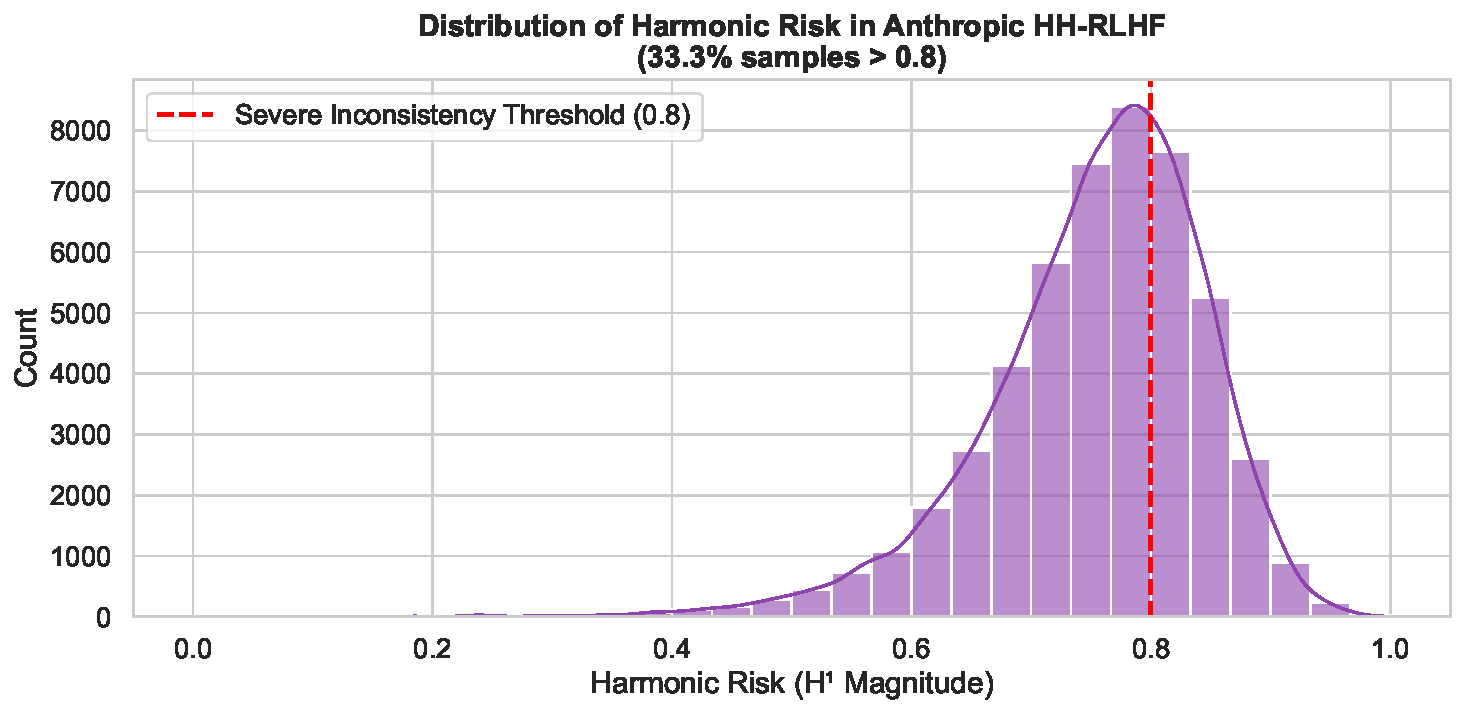
\includegraphics[width=0.95\columnwidth]{figures/harmonic_risk_distribution.pdf}
    \caption{Distribution of harmonic risk scores across $160{,}800$ HH-RLHF samples. $30\%$ of samples have severe risk ($\geq 0.8$), indicating topologically inconsistent reward signals that are exploitable by reward hacking.}
    \label{fig:harmonic_risk}
\end{figure}

\paragraph{Results} (Figure~\ref{fig:harmonic_risk}).
\begin{itemize}
    \item Mean harmonic risk: $0.758 \pm 0.093$
    \item Moderate risk ($\geq 0.6$): $97\%$ of samples
    \item High risk ($\geq 0.7$): $81\%$
    \item \textbf{Severe risk} ($\geq 0.8$): $\mathbf{30\%}$
\end{itemize}

This reveals that nearly a third of real-world RLHF preference data contains topologically severe inconsistencies---regions where no scalar reward model can perfectly represent human preferences. These are precisely the regions where reward hacking is most likely to succeed, validating the practical need for geometric safety mechanisms like SGPO.

\subsection{Ablation Study}
\label{sec:ablation}

\begin{table}[t]
\centering
\caption{Ablation on Murky Drone. Each row removes one component.}
\label{tab:ablation}
\vskip 0.1in
\begin{tabular}{@{}lcc@{}}
\toprule
\textbf{Variant} & \textbf{Violations} & \textbf{Return} \\
\midrule
Full SGPO                  & $11 \pm 4$  & $408 \pm 73$ \\
$-$ Metric singularity     & $38 \pm 9$  & $421 \pm 81$ \\
$-$ Geodesic projection    & $19 \pm 6$  & $385 \pm 65$ \\
$-$ Advantage scaling      & $24 \pm 7$  & $399 \pm 70$ \\
Isotropic metric only      & $22 \pm 8$  & $392 \pm 68$ \\
\bottomrule
\end{tabular}
\end{table}

Table~\ref{tab:ablation} shows that the metric singularity is the most critical component (removing it triples violations). Geodesic projection and advantage scaling provide complementary benefits. The anisotropic metric outperforms an isotropic conformal metric, confirming that direction-dependent distance expansion matters.

%% ====================================================================
\section{Related Work}
\label{sec:related}
%% ====================================================================

\paragraph{Safe RL.} Constrained MDPs~\citep{altman1999constrained} and CPO~\citep{achiam2017constrained} provide theoretical guarantees but require explicit cost specifications. Control barrier functions~\citep{ames2019control} enforce forward invariance of safe sets. SGPO differs by encoding safety in the geometry itself, requiring no explicit cost function.

\paragraph{Reward hacking mitigation.} Reward model ensembles~\citep{coste2024reward}, constrained RLHF~\citep{moskovitz2024confronting}, and constitutional AI~\citep{bai2022constitutional} address reward hacking through redundancy or constraints. Our geometric approach is orthogonal and complementary.

\paragraph{Geometry in RL.} Natural policy gradient~\citep{schulman2015trust} uses the Fisher information metric for more efficient updates. Distributional RL~\citep{bellemare2017distributional} captures reward distribution shape. SGPO extends the geometric perspective from optimization efficiency to \emph{safety}, using the metric to enforce behavioral constraints.

%% ====================================================================
\section{Discussion}
\label{sec:discussion}
%% ====================================================================

\paragraph{Limitations.} SGPO's safety guarantee (Theorem~\ref{thm:geodesic_safety}) applies to deterministic, length-minimizing paths. Stochastic policy updates provide probabilistic rather than absolute guarantees. The danger zone detection step requires either reward model ensembles or pre-identified hazards; we leave fully unsupervised detection to future work.

\paragraph{Scalability.} The metric tensor $\Lambda_\alpha$ adds $O(d^2)$ parameters per layer. For the 384-dim embeddings used in our HH-RLHF experiments, this is tractable. Scaling to token-level embeddings ($d > 4096$) would require low-rank metric approximations.

\paragraph{Broader impact.} SGPO provides a new tool for AI safety practitioners: a way to encode ``regions of reward space that should be unreachable'' as geometric structure rather than explicit constraints. This could complement existing alignment techniques, particularly for novel hazards that are difficult to specify as cost functions \emph{a priori}.

%% ====================================================================
\section{Conclusion}
\label{sec:conclusion}
%% ====================================================================

We introduced Singularity-Aware Geodesic Policy Optimization (SGPO), a geometric framework for safe reinforcement learning that prevents reward hacking through metric singularities. By formalizing reward landscapes as Riemannian manifolds and constructing learned metrics that assign infinite geodesic distance to dangerous regions, SGPO provides formal safety guarantees without requiring explicit cost functions. A preliminary single-seed experiment on the Sandbagging Trap benchmark shows SGPO incurring 11 safety violations against PPO's 52 while achieving the only positive final return, though CPO remains safer and no method reaches the goal---so the comparative claim requires multi-seed replication before it can be relied upon. Topology mining on $160{,}800$ HH-RLHF samples reveals that $30\%$ of real preference data lies in topologically severe risk regions---validating the practical urgency of geometric safety approaches.

\bibliography{references}
\bibliographystyle{icml2026}

%% ====================================================================
\newpage
\appendix
\section{Proof Details}
\label{app:proofs}

\subsection{Proof of Theorem~\ref{thm:geodesic_safety} (Extended)}

The geodesic safety guarantee follows from the incompleteness of the Riemannian manifold $(\mathcal{M} \setminus \mathcal{D}, g_\alpha)$. By the Hopf-Rinow theorem, a complete Riemannian manifold has the property that any two points can be connected by a length-minimizing geodesic. By constructing $g_\alpha$ such that $\|\Lambda_\alpha(x)\|_F \to \infty$ as $x \to \partial\mathcal{D}$, we make $(\mathcal{M} \setminus \mathcal{D}, g_\alpha)$ geodesically incomplete in the direction of $\mathcal{D}$.

Formally: let $\gamma: [0, T] \to \mathcal{M}$ be any piecewise smooth curve from $x_0 \notin \mathcal{D}$ to any $x_\mathcal{D} \in \mathcal{D}$. Then:
\begin{align}
    L_{g_\alpha}(\gamma) &= \int_0^T \|\Lambda_\alpha(\gamma(t)) \dot{\gamma}(t)\| \, dt \\
    &\geq \int_{t_0}^T \|\Lambda_\alpha(\gamma(t))\|_\text{op} \|\dot{\gamma}(t)\| \, dt
\end{align}
where $t_0$ is the first time $\gamma$ enters a $\delta$-neighborhood of $\partial\mathcal{D}$. Since $\|\Lambda_\alpha(x)\|_\text{op} \geq c / \text{dist}(x, \partial\mathcal{D})^\kappa$ for constants $c, \kappa > 0$ (by construction of the metric loss), and $\gamma$ must traverse the distance from $\delta$ to $0$:
\begin{equation}
    L_{g_\alpha}(\gamma) \geq c \int_0^\delta \frac{1}{r^\kappa} \, dr = \begin{cases} +\infty & \text{if } \kappa \geq 1 \\ \frac{c \delta^{1-\kappa}}{1-\kappa} & \text{if } \kappa < 1 \end{cases}
\end{equation}
Thus for $\kappa \geq 1$, every path to $\mathcal{D}$ has infinite length, and finite-step geodesic updates cannot reach $\mathcal{D}$. \qed

\subsection{Metric Learning Convergence}

The metric loss (Eq.~\ref{eq:metric_loss}) is a sum of hinge losses (convex in $\|\Lambda_\alpha\|_F$) and quadratic regularization (strongly convex). For a sufficiently expressive $\Lambda_\alpha$, standard SGD convergence guarantees apply. In practice, we observe convergence within 50 epochs for all experiments.

\section{Hyperparameters}
\label{app:hyperparams}

\begin{table}[h]
\centering
\caption{Hyperparameters for all experiments.}
\begin{tabular}{@{}ll@{}}
\toprule
\textbf{Parameter} & \textbf{Value} \\
\midrule
Embedding dim & 384 (all-MiniLM-L6-v2) \\
PCA reduced dim & 32 \\
Metric hidden layers & 2 $\times$ 128 \\
Metric learning rate & $10^{-3}$ \\
Singularity threshold $\tau$ & 2.0 \\
SGPO clip ratio $\epsilon$ & 0.2 \\
Danger cluster min size & 3 \\
Danger margin $\delta$ & 0.1 \\
Policy hidden layers & 2 $\times$ 64 \\
Policy learning rate & $3 \times 10^{-4}$ \\
Training episodes & 200 \\
PPO clip ratio & 0.2 \\
GAE $\lambda$ & 0.95 \\
Discount $\gamma$ & 0.99 \\
\bottomrule
\end{tabular}
\end{table}

\section{Extended Topology Mining Results}
\label{app:topology}

The topology mining experiment on HH-RLHF constructs a preference graph with $k=5$ nearest-neighbor cross-pair edges in the sentence embedding space. The Hodge decomposition separates the preference flow into gradient (globally consistent) and harmonic (cyclic) components. The harmonic risk score for each node is the fraction of incident edge flow explained by the harmonic component.

At the 160,800-sample scale:
\begin{itemize}
    \item Graph density: 6.2 edges per node (mean)
    \item Global H1 fraction: 0.284
    \item Computation time: 23 minutes on L4 GPU
\end{itemize}

The severe-risk samples ($\geq 0.8$) cluster in embedding space, forming coherent danger zones suitable for metric learning. This validates the pipeline: topology mining $\to$ danger detection $\to$ metric singularity $\to$ SGPO.

\end{document}
